\documentclass{ctexart}
\usepackage{amsmath}
\usepackage{amssymb}
\usepackage[a4paper, total={6in, 8in}]{geometry}
\usepackage{float}
\usepackage{subfigure}
\usepackage{graphicx}

\title{FEM - 第10周作业}
\author{SA23001071 杨哲睿}
\ctexset{
  section/format += \sffamily\raggedright,
}
\date{\today}

\begin{document}
\maketitle


\section{Introduction}
编写程序求解两点边值问题:
\begin{equation}
  \begin{cases}
    - \Delta u = f & (x, y) \in \Omega = [0, 1] \times [0, 1]\\
    u|_{\partial \Omega} = 0
  \end{cases}
\end{equation}
选取等距网格剖分,有限元空间选取分段线性多项式空间 $V_h$,选取准确解 $u(x,y) = (x-1) \sin (x) (y-1) \sin y$ 算出满足方程的$f(x, y)$。

\begin{eqnarray}
  f(x, y) = (-2\cos x- (x-1) \sin x) (y-1)\sin y + (-2\cos y-(y-1)\sin y)(x-1)\sin x
\end{eqnarray}

\section{Method}

定义双线性型$a(u, v) = \int_\Omega \nabla u \cdot \nabla v \mathrm dx$,
内积$(f, g) = \int_\Omega f \cdot g \mathrm dx$。那么变分问题是

\textit{找 $u\in V = \{ v\in H^1[0, 1], v|_\Omega = 0\}$,使得$a(u, v) = (f, v), ~ \forall v \in V$都成立.}


有限元空间为:
\begin{equation}
  V_h = \left\{v | v\in C(\Omega), v|_K \in P^2(K) , K \in \mathcal{T}_h, v| _{\partial \Omega} =0\right\}
\end{equation}

实验中采用三角网格划分,单元数为 $2N^2$ 如下,内部点数$(2N-1)^2$,边界点数$8N$。

\begin{figure}[H]
  \centering
  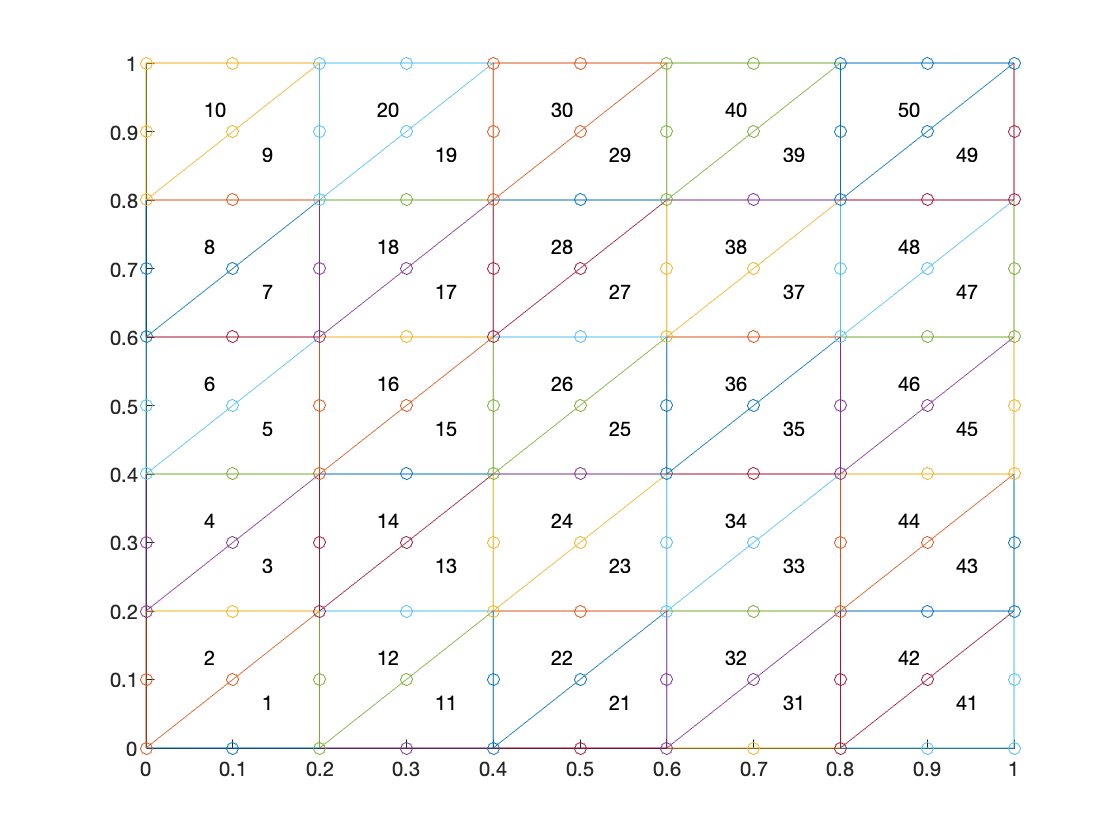
\includegraphics[width=0.8\linewidth]{mesh.png}
\end{figure}

对应的刚度矩阵为:
\begin{figure}[H]
  \centering
  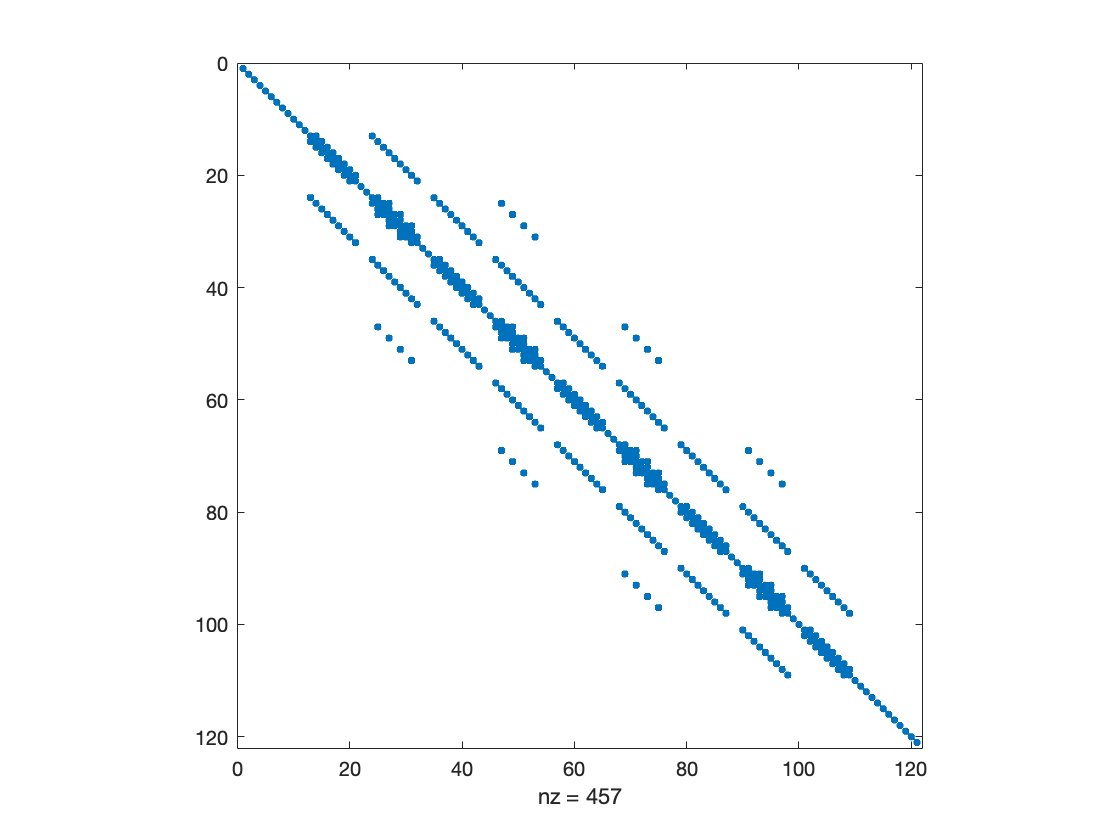
\includegraphics[width=0.65\linewidth]{./matrix.png}
\end{figure}

该刚度矩阵的构造采用了上课所说的第二种方法。先不考虑边界节点和内部点的区别,而直接构造刚度矩阵。由于我们采用的是零边界条件,所以可以将边界点$i$对应矩阵中的元素
\begin{equation}
  K_{i j} = K_{j i} = 0 \quad \forall i \ne j\quad K_{i i} = 1
\end{equation}
按照这样的规则进行赋值。

局部刚度矩阵的计算:由于我们选取的是相当规则的单元,因此其局部刚度矩阵是容易直接计算的。对于标准形函数

\begin{eqnarray}
  \bar \phi_1 = 2(1-x-y)(\frac{1}{2}-x-y)\\
  \bar \phi_2 = 4x(1-x-y)\\
  \bar \phi_3 = 2x(x-\frac{1}{2})\\
  \bar \phi_4 = 4xy\\
  \bar \phi_5 = 2y(y-\frac{1}{2})\\
  \bar \phi_6 = 4y(1-x-y)
\end{eqnarray}


其计算得到的矩阵为:
\begin{eqnarray}
  K = \left(\int_\Omega \nabla \bar\phi_i\cdot \nabla \bar\phi_j \mathrm dx\right) = 
  \begin{bmatrix}
    1 & -\frac{2}{3} & \frac{1}{6} & 0 & \frac{1}{6} & -\frac{2}{3} \\
    -\frac{2}{3} & \frac{8}{3} & -\frac{2}{3} & -\frac{4}{3} & 0 & 0 \\
    \frac{1}{6} & -\frac{2}{3} & \frac{1}{2} & 0 & 0 & 0 \\
    0 & -\frac{4}{3} & 0 & \frac{8}{3} & 0 & -\frac{4}{3} \\
    \frac{1}{6} & 0 & 0 & 0 & \frac{1}{2} & -\frac{2}{3} \\
    -\frac{2}{3} & 0 & 0 & -\frac{4}{3} & -\frac{2}{3} & \frac{8}{3} \\
  \end{bmatrix}
\end{eqnarray}
而经过变换后到局部基函数,所对应的矩阵也是完全相同的。以单元 1 为例。坐标变换为
\begin{equation}
  \phi = \bar\phi\left(1 - \frac{1}{h} x, \frac{1}{h} y\right)\\
\end{equation}
那么
\begin{equation}
  \begin{aligned}
    \frac{\partial \phi}{\partial x} &= - \frac{1}{h}\frac{\partial \bar \phi}{\partial x}\\
    \frac{\partial \phi}{\partial y} &= \frac{1}{h}\frac{\partial \bar \phi}{\partial y}\\
  \end{aligned}
\end{equation}
这说明了对于局部基函数:
\begin{equation}
  \int_\Omega \nabla \phi_i \cdot \nabla \phi_j \mathrm dx = \frac{1}{h^2} \int_\Omega \nabla \bar \phi_i\cdot \nabla \bar \phi_j \mathrm dx
\end{equation}
而三角形的面积恰好是 $\frac{1}{2h^2}$,因此如果我们合理地规划顶点,始终让直角边出现在三角形的第一个标号上,那么实际上每一个局部刚度矩阵就是$K$。这在构造稀疏矩阵系数时可以极大的简化操作。

\section{Results}

对于求得的系数,先进行Lagrange插值,然后进行梯形公式数值积分。可以看出,有限元方法的$L^2$误差是3阶的,$H^1$误差是2阶的。
\begin{table}[H]
  \caption{\label{table.label} 误差分析} \centering
  \bigskip
  \begin{small}
  \begin{tabular}{|c|c|c|cc|cc|}
    \hline
    网格总数 & 总内部结点数 & 总边界点数& $L^2 $ error & order &$ H^1$ error & order\\\hline
    200 & 361 & 80 & 9.7205e-7 & --- &  7.8018e-05 & --- \\
    800 & 1521 & 160 & 9.6136e-08 & 3.3379 & 1.761e-05 & 2.1474 \\
    3200 & 6241 & 320 & 1.0087e-8 & 3.2526 & 4.1409e-06 & 2.0884 \\
    12800& 25281 & 640 & 1.1216e-9 & 3.1689 & 1.0005e-6 & 2.0492 \\\hline
  \end{tabular}
  \end{small}
\end{table}

误差分析:因为选择了2次的Lagrange单元,那么它的插值误差是$O(h^3)$的,对于导数的误差是 $O(h^2)$ 这和我们计算得到的误差阶是相同的。

\end{document}
